\documentclass[12pt]{article}
\usepackage{amsmath}
\usepackage{amssymb}
\usepackage{graphicx}
\usepackage{tabulary}
\usepackage{float}


\begin{document}

\title{Homework 1 for Einstein group}%replace X with the appropriate number
\author{William Harrington, David Hernandez, Waleed Alhaddad\\ %replace with your name
ECE478} %if necessary, replace with your course title
 
\maketitle
\begin{description}
	\item[Introduction] \hfill \\ \\
		This report contains a detailed explanation of the homework 1 assignment for the Einstein group. \\ \\
		\textbf{Learning Outcomes} \hfill \\
		The purpose of this homework was to fulfill the following learning outcomes.
		\begin{enumerate}
			\item Use of Kinect to control a robot, to create commands and data for a robot.
			\item The concept of state machine in robotics
			\item The concept and use of fuzzy logic in robotics
			\item Using Powerpoint for scenario prototyping
			\item Dialogs with robots
		\end{enumerate}
		\newpage
		\textbf{First phase explanation} \hfill \\
		\begin{figure}[H]
			\caption{A high level diagram of the first phase objectives}
			\fbox{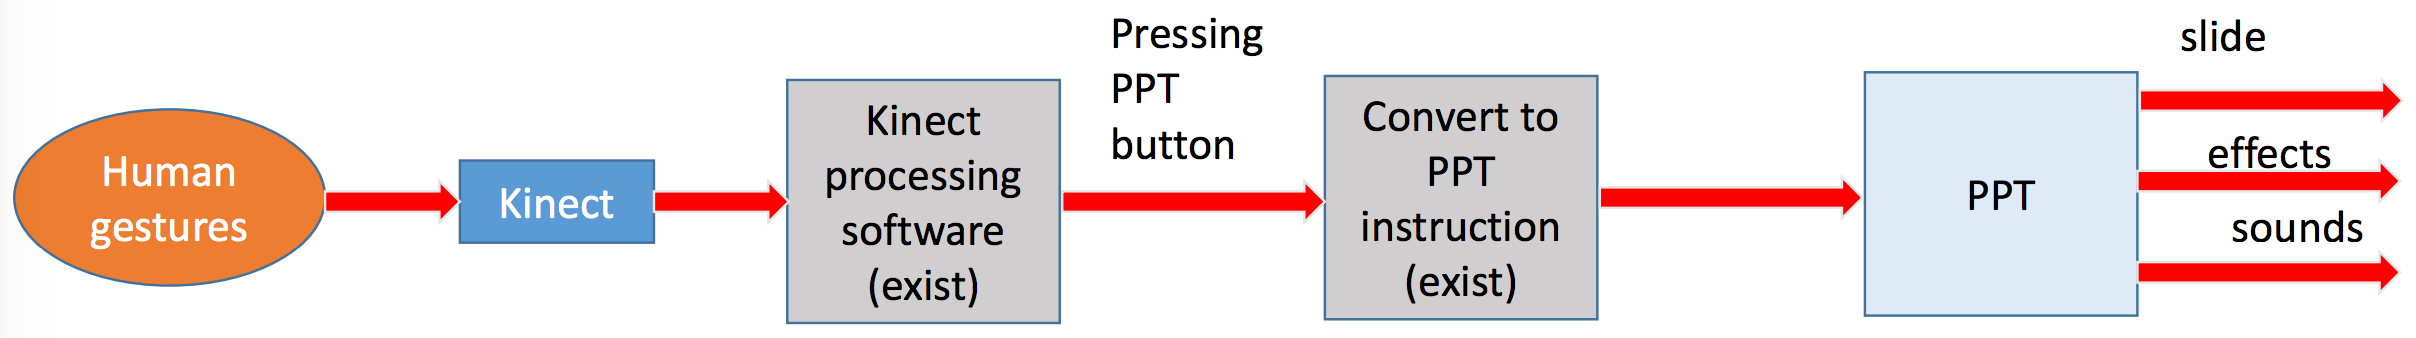
\includegraphics[scale=.3]{hw1_phase1_diagram.png}}
		\end{figure}
		\textbf{The objective for the first phase of this homework was to:}
		\begin{enumerate}
			\item Figure out how to use a Kinect to control the mouse on a computer 
			\item Figure out how to use Kinect to control a powerpoint presentation
			\item Create a powerpoint presentation with info, effects, figures, pictures, and videos about Einstein and the "Quantum Debate" play
			\item Record voice with German accent that is suppose to be Einstein for the powerpoint presentation
		\end{enumerate}
		\begin{enumerate}
			\item \textbf{Software to control mouse and powerpoint presentation with Kinect: \hfill \\
					$https://kinectmouse.codeplex.com/$}
			\item \textbf{Software for interacting with robot and powerpoint: \hfill \\
					$https://github.com/wrh2/ECE478/tree/master/Einstein$}
		\end{enumerate}		
\end{description}

\end{document}